\section{Usine Logicielle \& Katana}

\subsection{Usine Logicielle}
L'usine logicielle est l'ensemble de logiciels, d'outils et de procédures qui permettent de structurer et d'industrialiser les développements VSCT, ainsi que leur validation et déploiement sur l'infrastructure VSCT (hors VSCloud).

Dans sa définition actuelle : elle est la continuation de la nouvelle usine logicielle Lille et de Katana.

\begin{figure}[ht]
 \centering
 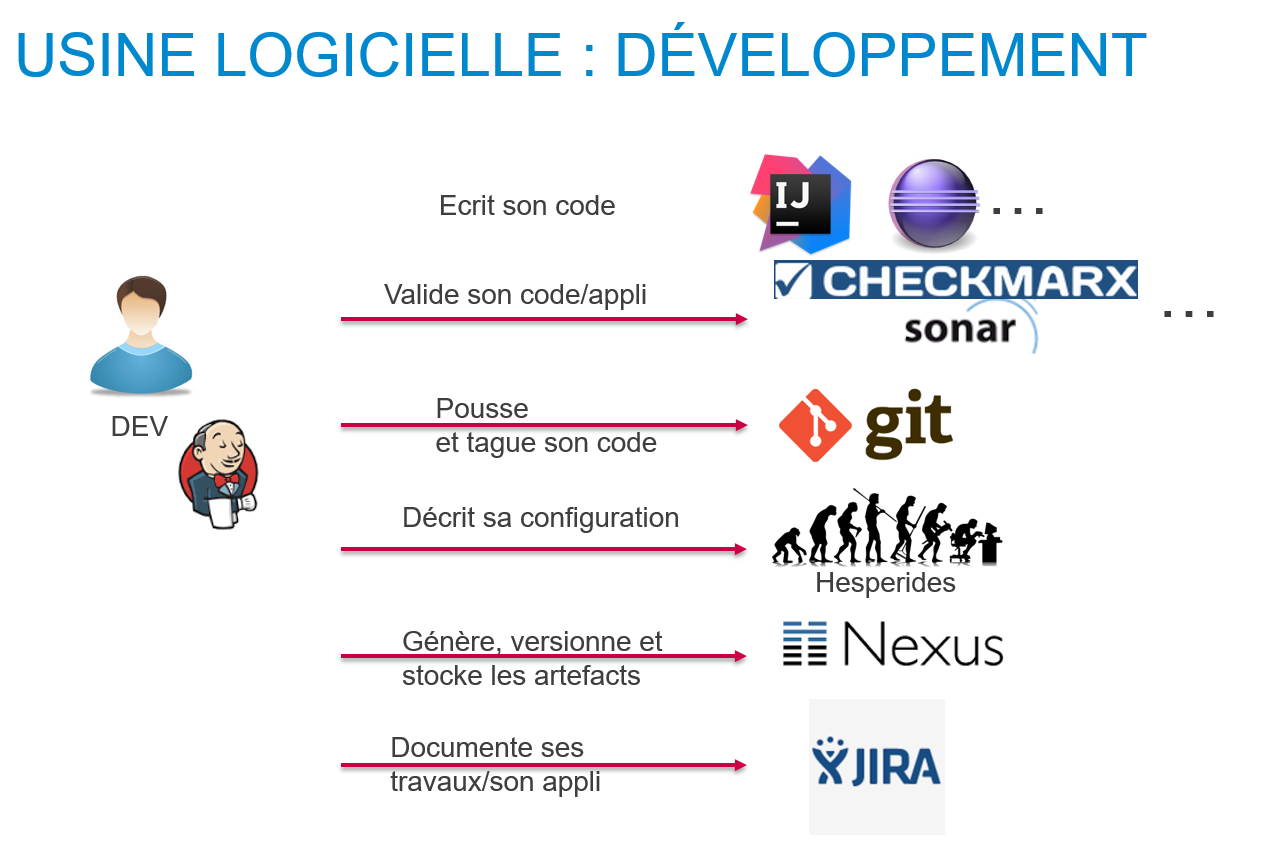
\includegraphics[width=0.8\textwidth]{usine-logicielle-developpement}
 \caption{Usine Logicielle: Développement}
\end{figure}

Le développeur édite ses sources sur son poste de travail et les versionne sous GIT, avec entreposage dans une forge GITLAB .

L'application fait elle-même l'objet de versions formalisées, avec les livrables individuels packagés et archivés sur un entrepôt de binaires (NEXUS).

Pour chaque application, plusieurs plateformes sont montées sur l'infrastructure pour installer l'application.

Chaque plateforme a un rôle défini. Les plateformes de production font l'objet d'une gestion spécifique, le plus souvent pilotée par les équipes d'exploitation.

Le développeur dispose d'un outillage d'intégration/déploiement continue (JENKINS) pour piloter les compilations/générations, validations, déploiements sur des plateforme intermédiaires...
Pour certaines de ces étapes, JENKINS pilote des outils-tiers (FISHEYE, CRUCIBLE, CHECKMARX, SONAR, etc).

Les serveurs (virtuels ou non) des plateformes sont accessibles en ligne de commande SSH au travers d'un frontal WALLIX, en fonction des droits de chacun.

Un frontal web (RUNDECK) permet de mettre à disposition des utilisateurs des opérations de plus haut-niveau, en self-service web sur les serveurs/plateformes (exemples : déploiement applicatif, reconfiguration applicative, arrêt/relance et autres opérations spécifiques sur les serveurs).

\begin{figure}[ht]
 \centering
 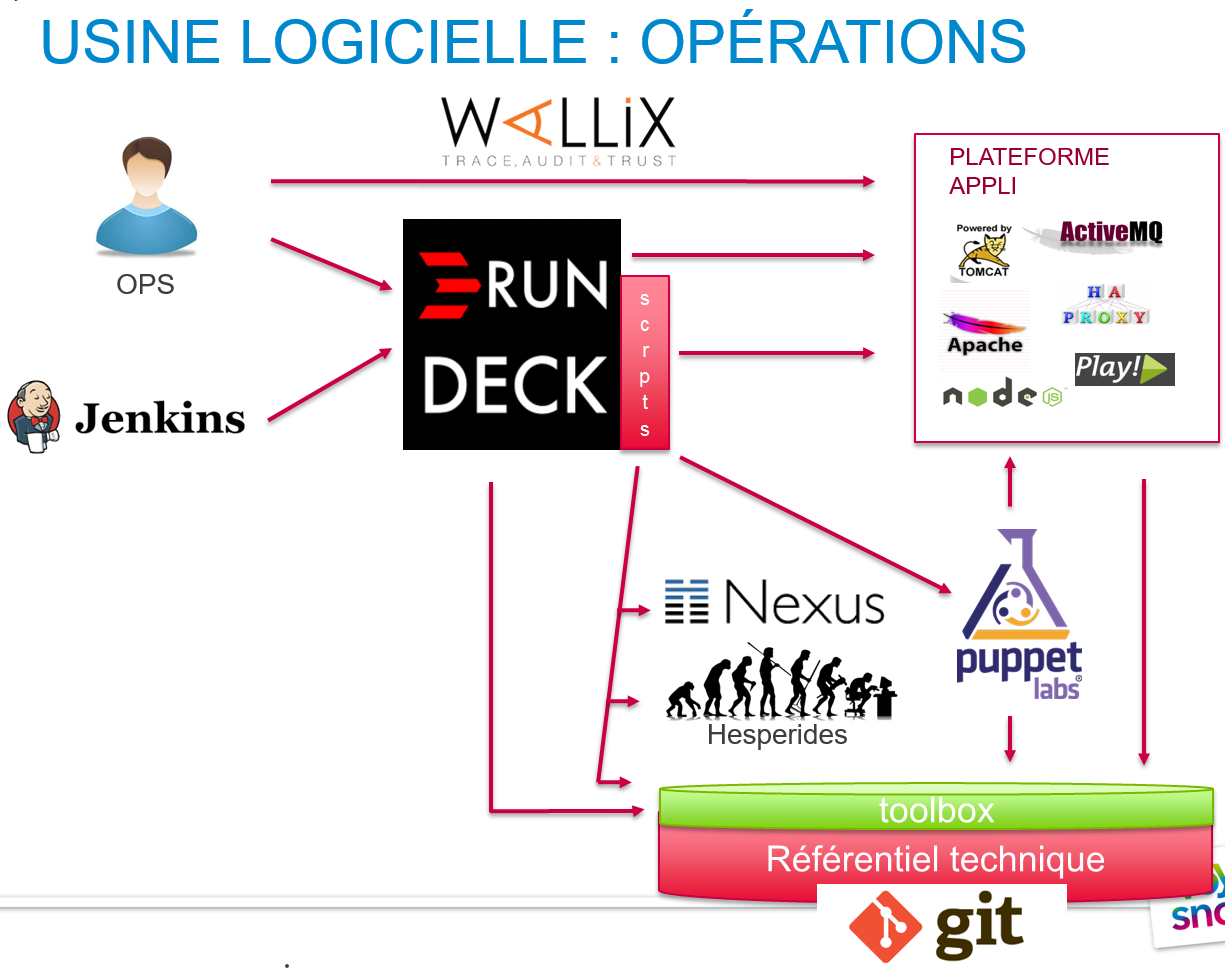
\includegraphics[width=0.8\textwidth]{usine-logicielle-operation}
 \caption{Usine Logicielle: Opération}
\end{figure}

La configuration détaillée des différentes plateformes de l'application est industrialisée par :
\begin{itemize}
 \item l'outil PUPPET (configuration technique - COTS) et un referentiel technique en infra-as-code ;
 \item l'outil HESPERIDES (configuration application - développement VSCT en open-source).
\end{itemize}

Sauf cas particulier, l'accès aux outils et aux plateformes se fait selon l'authentification Active Directory de l'utilisateur.
\subsection{Katana}

La solution Katana assure la configuration technique, le déploiement applicatif et autres tâches industrialisées sur les machines des infrastructures VSCT de Lille/St-Denis (DMZs hors-production, Assemblage, Perf, Partenaires, Rithmics, Technique, Production, SNB....), à l'exception notable des SIs du CNIT, de VSCloud et des infra Big Data.

\begin{figure}[ht]
 \centering
 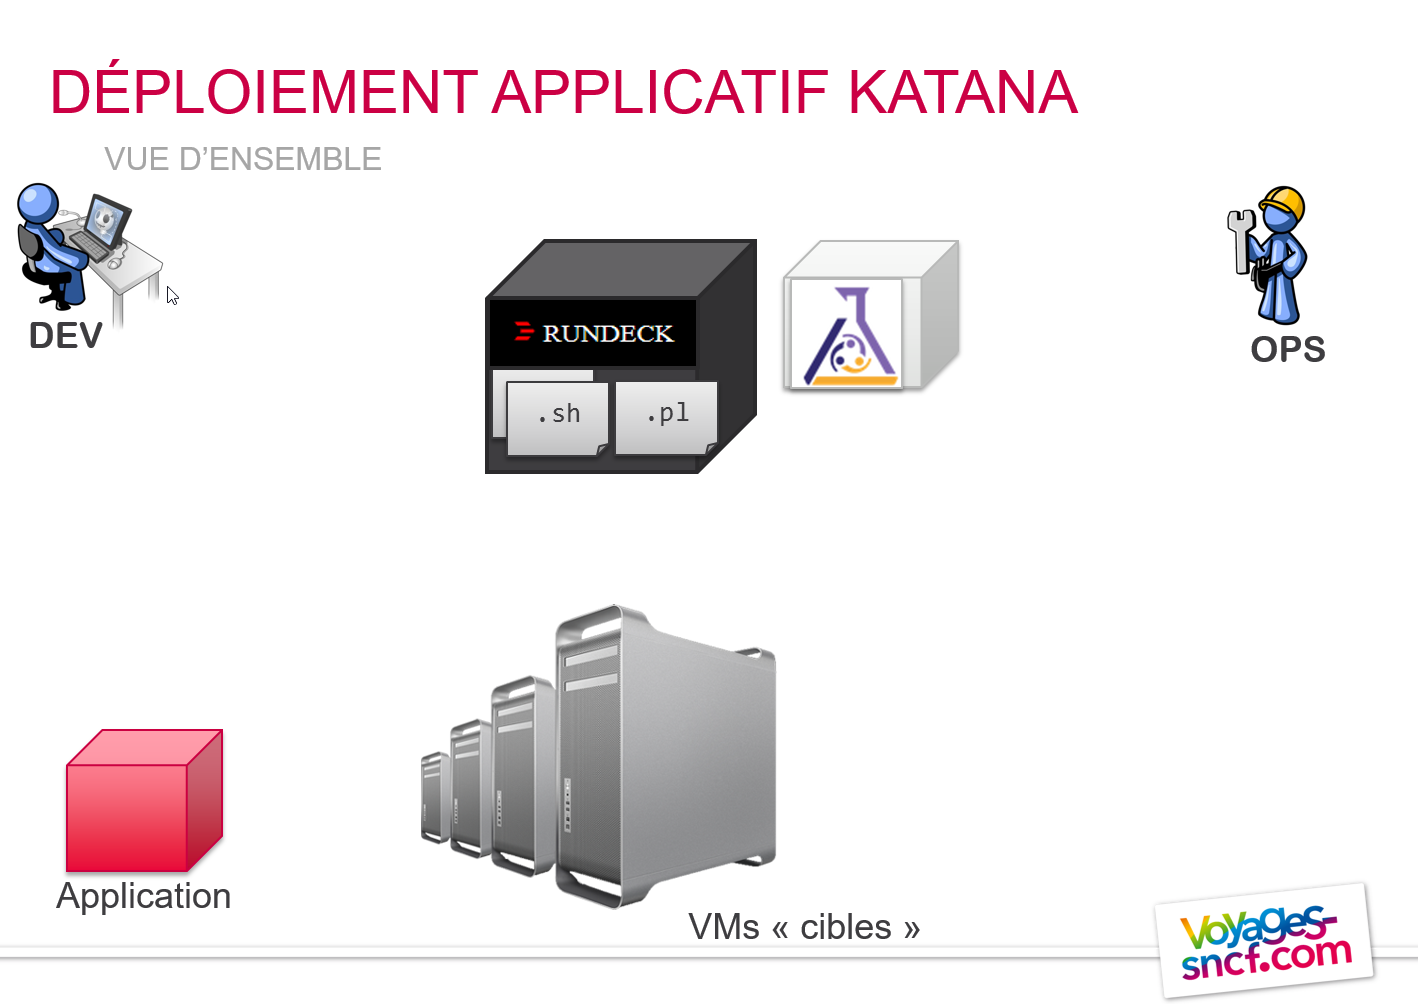
\includegraphics[width=0.8\textwidth]{katana}
 \caption{Déploiement Applicatif Katana}
\end{figure}

Elle est composée de :

\begin{itemize}
 \item un référentiel de données techniques sur les plateformes/machines sous forme infraAsCode (fichiers env Yaml pour les plateformes, fichiers de configuration Puppet);
 \item un référentiel des configurations applicatives: Hesperides (géré par sa propre communauté);
 \item un catalogue de scripts (bash/perl/groovy/...), issu des projets de déploiement VSCT, implantant les opérations de déploiement/contrôle/supervision/etc;
 \item un orchestrateur de tâches en self-service, Rundeck, qui pilote les tâches du Puppet et du catalogue de script (en central, ou sur les machines). Il peut être contrôlé soit manuellement (par son IHM web), soit par API REST.
\end{itemize}

Katana s'inscrit dans l'Usine Logicielle VSCT. La solution s'intègre en particulier avec les outils:
\begin{itemize}
 \item Jenkins: peut piloter l'orchestrateur de tâches dans le cadre des processus d'intégration ou de déploiement continus
 \item Nexus: pour le stockage des livrables applicatifs et autres artefacts (en particulier la note de livraison(lexique. \ref{lexi:delivery_note}), le catalogue de scripts, les projets rundeck...)
 \item GIT: pour le stockage et le versionnement des fichiers (code du catalogue de scripts, référentiels de données en Yaml, fichiers de configuration Puppet...)
\end{itemize}
